  \documentclass[AMA,STIX2COL]{WileyNJDv5}

\usepackage{etoolbox}
\usepackage{geometry} 
\usepackage{enumitem} 
 


\PassOptionsToPackage{dvipsnames}{xcolor}
\usepackage{xcolor}
\usepackage{colortbl}
\usepackage{listings}
\usepackage{fvextra}
\usepackage{fontspec}
\usepackage[font=small]{caption}
\hypersetup{hidelinks}
\setmonofont{Fira Code}

\newcommand{\IT}{{\sffamily EZR}}

% Colors
\definecolor{bggray}{gray}{0.98}
\definecolor{kwblue}{rgb}{0.1,0.2,0.7}
\definecolor{strgreen}{rgb}{0.0,0.6,0.3}
\definecolor{commentrust}{rgb}{0.6,0.2,0.1}
\definecolor{ident}{rgb}{0.1,0.1,0.1}

% --- Toggleable tiny boxed markers (black <-> Maroon) -----------------

\definecolor{Maroon}{RGB}{128,0,0}
\newif\ifcircledred
\circledredfalse

\newcommand{\circledblack}{\global\circledredfalse}
\newcommand{\circledred}{\global\circledredtrue}
\newcommand{\circledtoggle}{%
  \ifcircledred
    \global\circledredfalse
  \else
    \global\circledredtrue
  \fi
}

\DeclareRobustCommand*\circled[1]{%
  \setlength{\fboxsep}{1.2pt}%
  \ifcircledred
    \fcolorbox{Maroon}{Maroon}{\color{white}\tiny\bfseries #1}%
  \else
    \fcolorbox{black}{black}{\color{white}\tiny\bfseries #1}%
  \fi
}
\DeclareRobustCommand{\one}{\circled{1}}
\DeclareRobustCommand{\two}{\circled{2}}
\DeclareRobustCommand{\three}{\circled{3}}
% ----------------------------------------------------------------------
\usepackage{tabularx}
% nicer mono (pick ONE)
\setmonofont{JetBrains Mono} % crisp, modern
% \setmonofont{Iosevka}
% \setmonofont{IBM Plex Mono}
% \setmonofont{Inconsolata}

% stronger keyword color (RoyalBlue is from dvipsnames)
\definecolor{kwblue}{named}{RoyalBlue}

\lstdefinestyle{prettyPython}{
  language=Python,
  basicstyle=\fontsize{5.0}{5.8}\selectfont\ttfamily,
  keywordstyle=\color{kwblue}\bfseries,
  stringstyle=\color{strgreen},
  commentstyle=\color{commentrust}\itshape,
  identifierstyle=\color{ident},
  numberstyle=\fontsize{4.4}{5.0}\selectfont\color{gray},
  showstringspaces=false,
  breaklines=true,
  breakatwhitespace=true,
  columns=fullflexible,
  keepspaces=true,
  tabsize=2,
  frame=none,
  rulecolor=\color{gray},
  framerule=0.25pt,
  framesep=0.35em,
  aboveskip=0.6em,
  belowskip=0.6em,
  frameb=false,
  escapeinside={(*@}{@*)}  % <<<<<< changed from !! .. !!
}

\lstset{style=prettyPython}

\newcommand{\CODE}[1]{%
  \begin{listing}
  \begingroup
  \setlength{\fboxsep}{0pt}
  \colorbox{bggray}{%
    \begin{minipage}{\linewidth}
    \lstinputlisting[style=prettyPython]{src/#1}
    \vspace{-0.5em}\color{bggray}\rule{\linewidth}{0.5pt}
    \end{minipage}
  }
  \endgroup
  \caption{\texttt{#1}}
  \label{lst:#1}
  \end{listing}
}

\articletype{Research Paper}
\received{Date Month Year}
\revised{Date Month Year}
\accepted{Date Month Year}
\journal{Journal}
\volume{00}
\copyyear{2023}
\startpage{1}

\raggedbottom

\usepackage{booktabs}   % Required for \midrule
\usepackage{adjustbox}  % Required for the \begin{adjustbox} environment
\usepackage{array}      % Required to define the custom 'C' column type
\usepackage{xcolor}     % Required for the \BLUE text color command

\begin{document}

\title{Simpler AI via Small, Speedy Symbolic Scripts (the EZR toolkit) }

\author[1]{Tim Menzies}
 

\author[2]{Author Two}
 

\authormark{TAYLOR \textsc{et al.}}
\titlemark{Small Scripts for Symbolic AI: Why and How (an EZR approach)}

\address[1]{\orgdiv{Computer Science}, \orgname{NC STate}, \orgaddress{\state{North Carolina}, \country{USA}}}

\address[2]{\orgdiv{Department Name}, \orgname{Institution Name}, \orgaddress{\state{State Name}, \country{Country Name}}}
 

\corres{Corresponding author Tim Menzies,   \email{timm@ieee.org}}
 

%\fundingInfo{Text}
%\JELinfo{ejlje}

\abstract[Abstract]{Recent breakthroughs in AI have come from very complex models with trillions of parameters. This work has
overshadowed decades of work on   minimal AI.
Effective AI can be implemented, very simply, using symbolic methods. 
Lest we forget just how simple (and speedy) are symbolic methods,
this paper offers a tutorial
on  the EZR toolkit (a few hundreds likes of Python). 

EZR
has been tested on 127  tasks inclduing regression, prediction, optimization,
multi-objective optimization,
 configuration, performance tuning, 
hyperparameter optimization, 
 product line engineering, project health forecasting, defect prediction, software testing, software process and cost estimation, and cross-domain generalization datasets,
data generation, and text mining.

 For 127 tasks, small explainable and effective models can be built that are simple to code and require very few data labels.
 Depending on the task, these tiny
tools can be just as effective and 10,000 times faster than
alternative state-of-art methods.
 Interestingly, these tools blur the distinction between optimization and prediction — optimizers rely heavily on code developed for prediction and vice versa. Both results, we argue, follow from the use of succinct symbolic AI scripts.

EZR is recommended   for  any resource bound environment (e.g. Green/Edge engineering); 
when it is hard to access authorative labelled data; when developers want to understand their AI tools; when educators want to teach AI;  and  when researchers want to explore combinations of different methods.
EZR and its test data  are freely
available under a MIT license at github.com/timm/ezr  and github.com/timm/ezr/moot.}

\keywords{Software Engineering, AI Teaching,
Tool Design,
Composability,
Minimal Toolkits}

\jnlcitation{\cname{%
\author{Menzies T.},
\author{Author T}, 
\ctitle{Small Scripts for Symbolic AI: Why and How (an EZR approach)}} \cjournal{\it Software Practice and Experience.} \cvol{2025;00(00):1--18}.}

%\fontsize{9}{10.8}\selectfont

\maketitle   
\section{Introduction}\label{sec1}


% \begin{raggedleft}
% {\em ``XYZ is a wonderful thing for people whose role \\
% in life is to be on top of things. But not for me; my\\
% role is to be on the bottom of things.   I try to learn ... \\
% exhaustively; then  (summarize that for) people \\
%  who don't have time for such study.''\\
% -- Donald Knuth\\
% }
% \end{raggedleft}

To say the least, current software engineering literature is eager to explore
highly complex methods. Few-shot prompting has evolved into agentic workflows
where LLMs (large language models) with trillions of parameters orchestrate
multi-agent collaboration and repository-scale comprehension
\cite{ma2023scope,wang2022machine,Dong2025SurveyCodeAgents,DBLP:journals/corr/abs-2507-15003}.

\newtheorem{obs}{Observation}

But should we use LLMs all the time for all AI tasks?
There are compelling reasons to seek alternatives. Recent results,
discussed in {\S}2, show that many SE problems are inherently simpler than
these massive models imply:
\begin{quote}{\bf The Keys Effect:} 
{\em The effective state space of many SE tasks is far smaller than it appears.
Most of the state is controlled by a handful of \underline{\em key} variables.
Such state spaces can be navigated by a handful of lightweight probes
\cite{ganguly2025lowgodatalightse}.}
\end{quote}
To say that  another way, not every SE problem requires an LLM. This is a critical
observation because there are many reasons why LLM usage
is counter-indicated.
For example, not all environments can support massive models; edge
computing devices, for instance, often lack the compute and memory necessary
to run them.
Also,  the ``black box'' nature of LLMs prevents the generation of
reliable audit trails and causal explanations required in high-stakes domains
like law, medicine, and safety-critical systems~\cite{rudin2019explaining}. 
Further, as Table~\ref{cautions}
documents, LLMs suffer from well-known shortcomings: hallucinating facts,
regenerating bugs from training data, and erosion of   the shared
understanding that teams need to safely evolve their
code~\cite{CognitiveDebt}.

(Aside: Even if rapid advancements in the LLM field mitigate some of these
  flaws listed in  Table~\ref{cautions}, a fundamental scientific problem remains: these massive
models are poorly validated and prohibitively expensive to build or evaluate
at scale. Consequently, for researchers outside the commercial infrastructure
that produces them, reproducibility and replication are effectively
impossible. We are asked to trust, rather than verify.)

 

Accordingly, this paper investigates which AI tasks in SE can be implemented
without the staggering complexity of LLMs.
We describe a  ``simplicity first''
minimal AI toolkit called EZR\footnote{Install using {\tt pip install ezr} or download from \url{http://githib.com/timm/ezr}.}. EZR implements classical AI algorithms such as
regression tree learning, a Naive Bayes classifier, an active learner, various
clustering algorithms, and numerous optimizers. We built these incrementally:
algorithm $i+1$ attempts to reuse as much code as possible from algorithms
$[1..i]$. When faced with design alternatives, we rejected complex approaches
that performed no better than simpler ones\footnote{This
analysis led to decisions such as EZR's regression trees splitting numeric
columns at the median, rather than at the point that minimizes expected
variance as done in CART~\cite{brieman84}.}.


\begin{table}[!t]
\fontsize{8pt}{9.5pt}\selectfont
\captionsetup[table]{font=small}
\caption{Some of the reported issues with LLMs.}\label{cautions}
\begin{tabularx}{\columnwidth}{r|X}
 \textbf{Issue} & \textbf{Evidence} \\ \hline
 Hallucinations & $>50$\% of ChatGPT answers have incorrect
 info \cite{S12} \\
 Human error & Humans overlook AI errors 39\% of the time
 \cite{S12} \\
 Bad code suggestions & 70\% faulty: 29\% correct, 51\% partial, 20\%
 wrong \cite{S15} \\
 Expert caution & Google coders use $\le 25\%$ of AI
 suggestions \cite{tabachnyk22completion} \\
 Training bias & LLMs regenerate bugs from training data
 \cite{S13} \\
 Energy & High consumption.   \\
 Explanation & Subsymbolic so  no causal/ explanatory reasoning.   
 Hard to debug/edit auto-generated code.   \\
 Verification & Prompt output is rarely verified  \\
 Planning & "Vibe coding" = no planning, more test
 costs  \\
 Ownership & Copy-pasting reduces developer job satisfaction  \\
 Bubble burst &  Withdrawal of investor capital?  \\
 Subsidies? & If capital moves, will LLM costs rise 10x--100x ? \\
 Cognitive debt & Generative and agentic AI let teams move fast
 while quietly eroding shared understanding of why systems are
 designed as they are \cite{CognitiveDebt}\\
 Maintenance & Lack of "under-the-hood" skills $\rightarrow$   
 disasters? \\ \hline
\end{tabularx}
\end{table}

All the data used to evaluate EZR is available on-line for other researchers
to repeat, improve and/or refute our findings.
That data, from the  MOOT
repository\footnote{URL: \url{http://github.com/timm/moot}; 
DOI: \url{https://doi.org/10.5281/zenodo.17354083}; 
ZENODO: \url{https://zenodo.org/records/17354083}} inclidudes 127 tasks 
including regress,ion prediction, optimization, multi-objective optimization, configuration, performance tuning, hyperparameter optimization, product line engineering, project
health forecasting, defect prediction, software testing, software process and cost estimation, cross-domain generalization datasets, data generation, and text mining.  For more on MOOT, see \S\ref{moot}.


From this effort, we observed several key findings.
Across 127 tasks:
\begin{itemize}
\item
Small explainable and effective AI models can usually be built that are simple to code and require very few data labels. 
\item Depending on the task, these tiny tools can be just as effective and 10,000 times faster than alternative state-of-the-art methods. Concretely: symbolic models can achieve optimizations within 80\% of the best possible outcome; effective models can be built from minimal labeled training data; and models requiring fewer than 10 features are highly sufficient, even on tasks with up to 1,000 input features. 
\item
All of this required surprisingly little code-- roughly 800 lines of Python, half of which comprise a test suite. This brevity is partly explained by the fact that optimizers and classifiers share far more infrastructure than is commonly assumed: once the core data structures are in place (a single \texttt{DATA} class powering classifiers, optimizers, and active learners alike), the boundary between optimization and prediction largely dissolves.
\end{itemize}
A standard objection to simple methods like EZR is that while they may be attractive for their brevity, they underperform more sophisticated alternatives when it matters. We therefore close this paper with a case study that directly addresses that objection: relevancy filtering in text mining
(task routinely handled with LLMs and embeddings)  can be performed surprisingly well with a simple variant of a standard Bayes classifier, at a fraction of the complexity and cost.

 

Before proceeding, we must delineate the scope of this paper's contributions.
{\bf Firstly},
 while our previous work introduced the foundational concepts of MOOT and EZR,
establishing the baseline efficacy of our symbolic models. That
prior work reported results 1a and 1c and all the other findings are new
for this paper.  


{\bf Secondly}, aligned with the core focus of \textit{Software: Practice 
and Experience}, this paper pivots from merely evaluating predictive 
performance to examining system design. Here, we provide a comprehensive deep 
dive into the EZR codebase. By detailing the architectural decisions, shared
data structures, and implementation pragmatics, we demonstrate exactly how to 
build and maintain an effective, resource-light AI toolkit for software 
engineering practitioners.
 
{\bf Thirdly}, this paper shows that    specific AI tasks can be radically simplified with a very simple code base.
This is \underline{\bf not} to say that 
 large models are somehow obsolete.  As mentioned above,
 LLMs remain   necessary for
  generative and unstructured tasks, such as natural language translation,
  dialogue generation, text summarization, and extracting semantic meaning
  from heterogeneous sources. However, our results
  do suggest that   many SE
  tasks have enough inherent structure  such that trillion-parameter models are an unnecessary 
    overcomplication. The boundary of where ``simplicity first'' fails
  remains an open question, but this paper proves that its reach is far broader
  than current literature assumes.

  
 
 


\begin{table}[!t]
\caption{Less is more?}\label{less}
\fontsize{8pt}{9.5pt}\selectfont
\begin{tabular}{p{.95\columnwidth}}\hline
\begin{itemize}[nosep, topsep=2pt, partopsep=0pt, leftmargin=*]
\item PCA projects data onto a few principal components~\cite{pca}; 
\item Amarel's 
theorem provers exploited ``narrows''i.e. small
regions of key decisions surrounded by a large space of irrelevancies~\cite{Amarel1986}; 
\item Chang
optimized nearest neighbor  using just a few exemplars~\cite{chang74};
\item The Johnson–Lindenstrauss lemma shows that random projection of $N$ dimensions 
to a smaller set of $O(\varepsilon^{-2}\log n)$ dimensions preserves pairwise distances within $(1\pm\varepsilon)$~\cite{johnson1984extensions}; 
\item The ATMS solved diagnosis problems by focusing on
a small number of  core assumptions~\cite{atms}; 
\item ISAMPLING solved large problems via just a few restarts~\cite{Crawford:1994}; 
\item Sparse coding yields efficient, low-dimensional data representations~\cite{olshausen2004sparse}; 
\item Feature selection research routinely  discarded up to 80\% of features~\cite{kohavi97}; 
\item theorem prover runtimes can be    reduced from  exponential   to polynomial by first  setting just a few ``backdoors''~\cite{backdoor}; 
\item Semi-supervised learning methods label much of the data using information
for a small   lower-dimensional  manifold~\cite{zhu05}; 
\item Active learning works by querying only a  few informative examples~\cite{settles2009active}; 
\item Optimization research found that probes of simple surrogates (built from very little data) was an effective optimization strategy~\cite{zul13,guo13};   
\item Model distillation work showed that   large LLMs can be compressed to something much smaller with negligible performance loss~\cite{shi22,yang24}. 
\end{itemize}\\\hline
\end{tabular}
\end{table}
\section{Background}
\subsection{Motivation}
 To  motivate our exploration of simple methods, this section notes that for thousands of years, many researchers
 have argued from something like the   keys effect
discussed in the introduction.
For example,
Ptolemy (100-170 AD) proposed that  phenomena should be explained by "the simplest hypothesis possible". 
 William of Occam (1361-1420 AD) warned that "entities must not be multiplied beyond necessity." The benefits of such simplicity are well-documented: lower compute and energy costs~\cite{calrero15,monserrate2022cloud}, easier explanation~\cite{veerappa2011understanding}, and faster tuning~\cite{fu2016tuning}. 
 Simpler models are also recommended for mission/safety-critical applications. For example, Rudin~\cite{rudin2019stop} argues convincingly that we should
{\em ``stop explaining black box machine learning models for high stakes decisions and use interpretable models instead.''}.

As Table~\ref{less} illustrates, the history of computing is replete with
examples of complex systems being radically simplified without sacrificing
performance.


\begin{table}[!t]
\captionsetup[table]{font=small}
\caption{When  simpler   outperforms complex (in SE).}\label{less1}
\fontsize{8pt}{9.5pt}\selectfont
\begin{tabular}{p{2.3cm}@{:~}p{5.6cm}}\hline
%\textbf{Application} & \textbf{Finding} \\ \hline
Text mining & When ranking terms used for bug severity (in error reports), then (a)~three terms were enough to classify the bug reports;
(b)~classifiers based on more terms performed no better~\cite{MenziesM08}.\\
Defect prediction1 & Predictions from 50 examples
performed just as well as using 500 or 5,000 examples~\cite{menzies2008implications}.\\
Defect prediction2
  & K-Means pre-clustering matched deep learning
    at 500$\times$ speedup~\cite{majumder2018500+}. \\
    Effort estimation
  & Traditional text mining methods (SVM+TFIDF) defeat deep learners and ran
    100$\times$ faster~\cite{Tawosi23}. \\
Data synthesis
  & Parametric statistics equalled GANs with
    less compute~\cite{Ling24} .\\
Hyperparameter \newline optimization.
  & For many SE analytics tasks, very fast tuning worked as well as
    more complex methods~\cite{Fu17,agrawal2019dodge}. \\
Tabular data
  & Tree-based models outperform deep nets
    on medium-sized tables~\cite{grinsztajn2022why}. \\
Configuration & For find the parameter settings that most improve software performance, a simple two-class Bayes classifiers performs just as well as ensembles of 100+ regression trees~\cite{ganguly2025lowgodatalightse}.\\
Search waste &  SE data forms sparse, isolated clusters~\cite{ganguly2025lowgodatalightse}. 
 Continuous searches (e.g., Adam) wastes time
 wandering over the empty space between sparse clusters. Stochastic jumps are better~\cite{ganguly2025lowgodatalightse}. \\\hline
\end{tabular}
\end{table}
 Table~\ref{less1} reports the same effect, this time focusing on the specifc domain of software engineering. 
  Strangely, in the domain of SE,   this lesson goes mostly unheeded. A survey of 229 SE papers using LLMs found that only 5\% compared against a simpler baseline~\cite{Hou24},  even though simpler methods routinely match or beat state-of-the-art performance while running 100x–1000x faster~\cite{majumder2018500+,ganguly2025lowgodatalightse,grinsztajn2022why,Tawosi23,Ling24,Fu17}. We conjecture this reflects a cognitive bias: Adams and Fillon et al.~\cite{adams2021people,Fillon25} found that across 400+ subjects given design tasks, people are four times more likely to select additive changes than
   subtractive changes even when the subtractive change is just as effective. That is, left to themselves,
{\em humans needlessly complicate their designs.}


Perhaps what is missing are exemplars — existence proofs that simple symbolic AI is not just theoretically attractive but practically effective. Hence this paper.


% ding from thise work is  the 
% inference machinery is largely    shared across   tasks. For example,
% \begin{itemize}
% \item
% Coding a nearest-neighbor classifier provided nearly everything needed for stochastic optimization.
% \item 
% Coding an optimizer provided nearly everything needed for software configuration and tuning.
% \end{itemize}
% This convergence suggests a radical reframing — rather than a zoo of specialized algorithms, AI may reduce to a handful of core operations, each "different" technique merely a thin variation on the same kernel. The field has been making things harder than they need to be. EZR is an existence proof that a simpler foundation is both possible and practical.

% \subsection{The Case for Simple Methods}
 
% Simplicity is no new idea. Ptolemy~(130~A.D.) urged
% explaining phenomena by ``the simplest hypothesis
% possible.'' William of Occam warned that entities must
% not be multiplied beyond necessity. The documented benefits
% are concrete: lower compute and energy
% costs~\cite{calrero15,monserrate2022cloud}, easier
% explanation~\cite{veerappa2011understanding}, and faster
% tuning~\cite{fu2016tuning}. Rudin~\cite{rudin2019stop}
% puts it plainly:
 
% \begin{quote}
% {\em ``Stop explaining black box machine learning models
% for high stakes decisions and use interpretable models
% instead.''}
% \end{quote}
 
\subsection{Test Data (from the MOOT repository)}\label{moot}


\newcolumntype{C}[1]{>{\centering\arraybackslash}p{#1}}
\begin{table*}[!t]
\fontsize{5pt}{6pt}\selectfont
\renewcommand{\baselinestretch}{0.7}
\caption{ MOOT's  127 SE optimization tasks. “x/y’’ denotes inputs/outputs (independent/dependent attributes).}
\label{combinedtable}
\begingroup
\scriptsize
\renewcommand{\arraystretch}{0.55}  % <<< SHRINK ROW HEIGHT

\begin{adjustbox}{max width=\textwidth}
\begin{tabular}{@{}C{1.4cm}@{~}p{2.5cm}p{3.9cm}p{4.0cm}p{1.1cm}p{1.4cm}c@{}}

\# Datasets & Dataset Type                     & File Names                                                               & Primary Objective                                                     & x/y          & \# Rows & Cited By       \\ \midrule
\rowcolor{blue!10} 25          & \begin{tabular}[c]{@{}l@{}}Specific Software\\Configurations\end{tabular} & SS-A to SS-X, billing10k                                                 & Optimize software system settings                                     & 3-88/2-3   & 197–86,059 & \cite{Amiraliminimaldata, menzies2025the, lustossa2024isneak, senthilkumar2024can, lusstosa2025less, nairMSR18, peng2023veer,nair2017using}   \\ 
\rowcolor{blue!10} 12          & \begin{tabular}[c]{@{}l@{}}PromiseTune Software\\Configurations\end{tabular} & \begin{tabular}[c]{@{}l@{}} 7
z, BDBC, HSQLDB, LLVM, \\ PostgreSQL, dconvert, deeparch,\\  exastencils, javagc,   redis, storm, x264
\end{tabular}                                                 & Software performance optimization                                     &  9-35/1  &  864-166,975 &  \cite{chen2026promisetune, chen2025accuracy, DBLP:conf/icse/XiangChen26, DBLP:journals/pacmse/Gong024, gong2024dividable} \\  
1           & Cloud                            & HSMGP num                                                                & Hazardous Software, Management Program data                           & 14/1         & 3,457 &  \cite{Amiraliminimaldata, menzies2025the, chen2025accuracy, senthilkumar2024can}     \\
1           & Cloud                            & Apache AllMeasurements                                                   & Apache server performance optimization                                & 9/1          & 192  &    \cite{Amiraliminimaldata, menzies2025the, chen2025accuracy, senthilkumar2024can}     \\
1           & Cloud                            & SQL AllMeasurements                                                      & SQL database tuning                                                   & 39/1         & 4,654 &    \cite{Amiraliminimaldata, menzies2025the, senthilkumar2024can}    \\
1           & Cloud                            & X264 AllMeasurements                                                     & Video encoding optimization                                           & 16/1         & 1,153  &   \cite{Amiraliminimaldata, menzies2025the, senthilkumar2024can}   \\
7           & Cloud                            & (rs—sol—wc)*                                                             & misc configuration tasks                                              & 3-6/1      & 196–3,840 &  \cite{Amiraliminimaldata, menzies2025the, senthilkumar2024can, lusstosa2025less, nairMSR18}  \\ 
\rowcolor{blue!10} 35          & Software Project Health          & Health-ClosedIssues, -PRs, -Commits                                      & Predict project health and developer activity                         & 5/2-3      & 10,001    &   \cite{Amiraliminimaldata, menzies2025the, senthilkumar2024can, lusstosa2025less,lustosa2024learning} \\ 
3           & Scrum                            & Scrum1k, Scrum10k, Scrum100k                                             & Configurations of the scrum feature model                             & 124/3      & 1,001–100,001 & \cite{Amiraliminimaldata, menzies2025the, lusstosa2025less, lustossa2024isneak} \\  
\rowcolor{blue!10} 8           & Feature Models                   & FFM-*, FM-*                                                              & Optimize number of variables, constraints and Clause/Constraint ratio & 128-1,044/3 & 10,001  &  \cite{Amiraliminimaldata, menzies2025the, lusstosa2025less, lustossa2024isneak}    \\  
1 &	Software Process Model &	nasa93dem &	Optimize effort, defects, time and LOC	& 24/3 &	93  & \cite{menzies2025the, senthilkumar2024can, lusstosa2025less, lustosa2024learning}\\
1           & Software Process Model           & COC1000                                                                  & Optimize risk, effort, analyst experience, etc                        & 20/5         & 1,001    &  \cite{Amiraliminimaldata, menzies2025the, senthilkumar2024can, lustosa2024learning,chen2018beyond}   \\
4           & Software Process Model           & POM3 (A–D)                                                               & Balancing idle rates, completion rates and cost                       & 9/3          & 501–20,001   & \cite{menzies2025the, senthilkumar2024can, lusstosa2025less, lustosa2024learning, lustossa2024isneak}\\
4           & Software Process Model    & XOMO (Flight, Ground, OSP)                                               & Optimizing risk, effort, defects, and time                            & 27/4         & 10,001    &  \cite{menzies2025the, senthilkumar2024can, lusstosa2025less, lustosa2024learning, lustossa2024isneak,chen2018beyond}  \\  
\rowcolor{blue!10} 3           & Miscellaneous                             & auto93, Car\_price, Wine\_quality                                        & Miscellaneous                                                         & 5-38/2-5   & 205–1,600  &  \cite{Amiraliminimaldata, menzies2025the, senthilkumar2024can, lusstosa2025less, lustosa2024learning} \\ 
4           & Behavioral                       & all\_players, student\_dropout,\newline HR-employeeAttrition, player\_statistics & Analyze and predict behavioral patterns                              & 26-55/1-3  & 82–17,738   &    \cite{nyagami_fc25_kaggle_2025, abdullah0a_student_dropout_analysis_prediction_2025, die9origephit_fifa_wc_2022_complete_2025, pavansubhasht_ibm_hr_analytics_attrition_2025}\\  
\rowcolor{blue!10} 4           & Financial                        & BankChurners, home\_data, Loan, \newline Telco-Churn                              & Financial analysis and prediction                                     & 19-77/2-5  & 1,460–20,000 &    \cite{blastchar_telco_customer_churn_2025, lorenzozoppelletto_financial_risk_for_loan_approval_2025, dansbecker_home_data_for_ml_course_2025, sakshigoyal7_credit_card_customers_2020} \\  
3           & Human Health Data                & COVID19, Life\_Expectancy, \newline hospital\_Readmissions                        & Health-related analysis and prediction                                & 20-64/1-3  & 2,938–25,000 &     \cite{dansbecker_hospital_readmissions_2025, kumarajarshi_life_expectancy_who_2025, hendratno_2022}  \\  
\rowcolor{blue!10} 2           & Reinforcement Learning           & A2C\_Acrobot, A2C\_CartPole                                              & Reinforcement learning tasks                                          & 9-11/3-4   & 224–318  &     \\ 
5           & Sales                            & accessories, dress-up, Marketing\_Analytics, socks, wallpaper            & Sales analysis and prediction                                         & 14-31/1-8  & 247–2,206 &     \cite{jessicali9530_animal_crossing_new_horizons_nookplaza_dataset_2021, jackdaoud_marketing_data_2022, syedfaizanalii_car_price_dataset_cleaned_2025}  \\  
\rowcolor{blue!10} 2	& Software testing	& test120, test600	& Optimize the class	& 9/1	& 5,161 &\\ \midrule
% 8           & Text Mining                      & Hall, Kitchenham, Radjenovic, Wahono                                     & Text mining for primary study selection                               & 5-50 / 1     & 1,710–8,912   \\ \midrule

127         & \textbf{Total}                            &                                                                          &                                                                       &              &        &      
\end{tabular}
\end{adjustbox}
\endgroup
\end{table*}
 
To  test EZR, we use data from the  MOOT repository\footnote{http://github.com/timm/moot.
MOOT = \underline{m}any \underline{m}ultiple \underline{o}bjective
\underline{o}ptimization \underline{t}asks.} that  documents
over 120 tasks. These tasks span configuration tuning (e.g., compiler optimization),
project health forecasting (e.g., GitHub issue lifetime classification), product
line engineering (e.g., high-dimensional constraint satisfaction for Scrum
feature models), defect prediction and mitigation, and software process and cost
estimation. This data   was collected from the case study information seen in numerous recent SE papers published at senior venues\footnote{
ICSE, FSE, TSE, IST, EMSE, TOSEM, ASE, etc. \cite{chen2026promisetune, DBLP:conf/icse/WeberKSAS23,10172849,DBLP:conf/icse/HaZ19,nair2017using,DBLP:conf/sigsoft/JamshidiVKS18,chen2025accuracy,xia2020sequential,krishna2020whence,Chen19, krall2015gale,chen2018beyond,fu2016tuning,hulse2025shaky, peng2023veer,guo2018data,lustosa2024learning,nair2018faster}.}.
 To the best of our knowledge, MOOT is the largest and most varied
collection of real multi-objective optimization tasks in SE. Earlier
resources (e.g., SPLOT) were valuable but narrow and are now offline.
Toolkits like Pygmo or Platypus offer synthetic benchmarks like ZDT,
DTLZ, Rosenbrock's banana\footnote{
The banana is a task with a non-convex decision frontier; i.e.
minimize $\sum_{i=1}^{n-1} \left[ 100(x_{i+1} - x_i^2)^2 + (x_i - 1)^2
\right], \quad -2.048 \leq x_i \leq 2.048, \quad i = 1, \ldots, n$.
}. But it is somewhat bananas to expect synthetic problems to convince
hard-nosed business users. MOOT's datasets come from published SE
studies, real performance logs, cloud systems, defect predictors, and
tuning tasks where bad configurations cost time, money, and
credibility.
Each MOOT  task has:
\begin{itemize}
\item
One to 11 goals (median=3)
\item
3 to 10044 input variables (median=11) 
\item and   100 to over 100,000 instances (median=10,000).  
\end{itemize}

 

% JUst to say the obvious: MOOT is not one data source or one repository. Rather it is 


% To put these ideas to work we used the MOOT repository of
% multi-objective optimization
% tasks~\cite{menzies2026moot}. MOOT's 127 tasks span a
% wide range of SE challenges; Table~\ref{moot} summarises
% the diversity. Each task is a table of $x$ inputs and $y$
% goals; goal columns are annotated with $+/-$ to indicate
% maximize/minimize. Dataset sizes range from 93 to
% 166,975 rows; dimensionality ranges from 3 to 1,044
% independent variables; goal counts range from 1 to 8.
% This variety makes MOOT a demanding proving ground for
% any claim that simple methods suffice.
 
% One striking finding from our experience with MOOT is
% that the inference machinery is largely shared across
% tasks. For example:
% \begin{itemize}
% \item Coding a nearest-neighbor classifier provided nearly
%   everything needed for stochastic optimization.
% \item Coding an optimizer provided nearly everything needed
%   for software configuration and tuning.
% \end{itemize}
% This convergence suggests a radical reframing: rather than
% a zoo of specialized algorithms, AI may reduce to a
% handful of core operations, each ``different'' technique
% merely a thin variation on the same kernel. The field has
% been making things harder than they need to be.
% \texttt{tree.py} is an existence proof that a simpler
% foundation is both possible and practical.


 
% This paper asks: \textit{what can we learn about AI by building it 
% as simply as possible?} Three insights emerge:

% \begin{itemize}
% \item \textbf{Insight 1: Shared kernel.} Classifiers, optimizers, 
%       and configurators reduce to the same handful of operations. 
%       Much AI complexity is accidental.
% \item \textbf{Insight 2: Data hunger is a myth.} Across 127 SE 
%       tasks, a small fraction of available data suffices --- 
%       sometimes a handful of labeled examples is enough.
% \item \textbf{Insight 3: Simple transfers.} Symbolic methods built 
%       for one task generalize readily to others, because the 
%       underlying machinery is shared.
% \end{itemize}

% \noindent The contributions of this paper are:
% \begin{itemize}
% \item \textbf{A unifying implementation.} EZR ($\sim$300-line core, 
%       $\sim$60-line apps) shows that 127 SE tasks reduce to one 
%       small shared codebase (MIT license; \url{github.com/timm/ezr}).
% \item \textbf{An annotated walkthrough.} A code-level tour that makes 
%       the shared kernel thesis concrete and reproducible.
% \item \textbf{A new active learning result.} A handful of labeled 
%       examples yields $>$85\% recall and $<$20\% false alarms 
%       when screening thousands of documents --- no LLM required.
% \item \textbf{A challenge to the field.} Given that only 5\% of SE 
%       papers compare LLMs to simpler baselines~\cite{Hou24}, EZR 
%       provides those baselines, ready to use.
% \end{itemize}

% \noindent The remainder of this paper is structured as follows.
% \S\ref{sec:motivation} replays key results showing that simple 
% symbolic methods match state-of-the-art performance across a broad 
% benchmark.
% \S\ref{sec:kernel} presents the annotated EZR walkthrough, 
% organized around the shared kernel thesis.
% \S\ref{sec:al} reports the new active learning result.
% \S\ref{sec:discussion} discusses implications for SE research 
% and education.

% \section{RQ1: can all AI be simplified?}

% \noindent\textbf{RQ1: Can all AI tasks be simplified?} Not all — generative tasks still require LLMs. But we have good evidence that symbolic methods suffice for regression, prediction, optimization, multi-objective optimization, configuration, performance tuning, hyperparameter optimization, product line engineering, project health forecasting, defect prediction, software testing, cost estimation, cross-domain generalization, data generation, and text mining.
% We will not claim our methods work best on every task — the No Free Lunch theorem forbids it. But that theorem cuts both ways: no method works best on all future examples. The practical question is always how quickly you can assess whether a method is working and switch if it is not. Symbolic methods are far faster to evaluate than LLMs, so we recommend applying them first. If they fall short, you have lost little time. If they succeed, you may never need the heavyweight alternative.



 


\begin{table*}[t]
\caption{Jet Propulsion Lab, orbital space plan. Predictions of
effort, months, defects, risks associated with 10,000 random samples from possible
  product/process/personnel   options. Data generated by USC COCOMO models~\cite{boehm2000software}. 
  Model attributes described at right. Rows sorted top to bottom, most to least
  desirable (so lowest effort, month, defects, risks shown at top).}\label{jpl}
%\centering
\begin{tabular}{p{0.62\textwidth}p{0.35\textwidth}}
\resizebox{0.62\textwidth}{!}{%
\begin{tabular}{rrrr|rrrrrrrrl}
\multicolumn{4}{c|}{$y$ dependent goals}&\multicolumn{9}{c}{$x$ independent input choices}\\ 
\multicolumn{4}{c|}{~}\\
\texttt{EFFORT-} & \texttt{MONTHS-} & \texttt{DEFECTS-} & \texttt{RISKS-}
  & \texttt{KLOC} & \texttt{LTEx} & \texttt{PCON} & \texttt{RELY} & \texttt{SITE}
  & \texttt{ETAT} & \texttt{ACAP} & \texttt{RESL} & \texttt{\dots} \\
\hline
58.07 (0.00) & 12.59 (0.00) & 63.45 (0.00) & 1.07 (0.40) & 25.39 & 3.66 & 4.57 & 2.44
  & 5.82 & 5.55 & 4.19 & 2.24 & \ldots \\
369.35 (0.15) & 22.25 (0.38) & 3236.77 (0.13) & 0.54 (0.20) & 364.95 & 3.97 & 4.48
  & 2.85 & 2.37 & 3.67 & 4.14 & 1.05 & \ldots \\
326.75 (0.13) & 21.36 (0.34) & 4716.41 (0.19) & 1.07 (0.40) & 89.89 & 1.74 & 2.69
  & 2.58 & 2.34 & 2.60 & 4.00 & 4.74 & \ldots \\
619.07 (0.28) & 25.94 (0.52) & 3053.00 (0.12) & 0.27 (0.10) & 238.86 & 1.56 & 3.66
  & 3.28 & 4.18 & 1.46 & 4.86 & 3.14 & \ldots \\
690.49 (0.31) & 26.05 (0.52) & 2289.34 (0.09) & 0.00 (0.00) & 322.42 & 2.56 & 4.93
  & 3.36 & 4.70 & 1.35 & 3.42 & 3.81 & \ldots \\
514.27 (0.21) & 24.78 (0.47) & 8113.69 (0.33) & 0.80 (0.30) & 253.04 & 3.70 & 2.29
  & 2.38 & 1.25 & 3.21 & 4.85 & 2.46 & \ldots \\
458.50 (0.18) & 23.84 (0.43) & 2529.85 (0.10) & 2.15 (0.80) & 116.59 & 1.92 & 1.97
  & 2.55 & 4.59 & 5.30 & 4.01 & 2.94 & \ldots \\
646.08 (0.26) & 26.86 (0.55) & 5627.24 (0.23) & 0.54 (0.20) & 193.04 & 3.67 & 1.84
  & 2.59 & 2.20 & 4.61 & 4.74 & 4.33 & \ldots \\
619.07 (0.25) & 25.94 (0.50) & 3053.00 (0.12) & 0.27 (0.10) & 238.86 & 1.56 & 3.66
  & 3.28 & 4.18 & 1.46 & 4.86 & 3.14 & \ldots \\
811.49 (0.37) & 27.94 (0.60) & 10288.87 (0.42) & 2.68 (1.00) & 149.28 & 1.56 & 1.72
  & 1.50 & 2.90 & 3.74 & 4.88 & 3.77 & \ldots \\
983.75 (0.46) & 30.50 (0.70) & 8574.98 (0.35) & 0.00 (0.00) & 274.44 & 2.22 & 4.19
  & 2.91 & 5.29 & 3.86 & 3.65 & 1.70 & \ldots \\
1126.37 (0.53) & 32.22 (0.77) & 20401.13 (0.82) & 0.00 (0.00) & 312.22 & 1.68 & 4.16
  & 3.97 & 4.52 & 2.77 & 3.86 & 1.32 & \ldots \\
1257.88 (0.58) & 32.64 (0.79) & 21036.78 (0.84) & 1.07 (0.40) & 284.67 & 3.19 & 1.40
  & 1.01 & 2.86 & 3.07 & 3.78 & 2.02 & \ldots \\
1428.28 (0.65) & 33.66 (0.83) & 6966.66 (0.28) & 0.54 (0.20) & 281.03 & 2.19 & 1.36
  & 3.54 & 3.42 & 1.36 & 4.71 & 4.89 & \ldots \\
1461.54 (0.66) & 35.47 (0.91) & 9058.17 (0.37) & 0.00 (0.00) & 253.31 & 3.39 & 1.66
  & 3.43 & 5.44 & 3.34 & 3.17 & 1.29 & \ldots \\
1462.12 (0.68) & 34.38 (0.85) & 10552.97 (0.42) & 0.00 (0.00) & 353.56 & 3.30 & 1.60
  & 2.43 & 2.87 & 5.78 & 3.43 & 2.50 & \ldots \\
1799.66 (0.85) & 36.31 (0.93) & 14859.26 (0.59) & 1.07 (0.40) & 299.21 & 2.28 & 2.17
  & 3.00 & 2.07 & 1.32 & 5.00 & 1.69 & \ldots \\
1796.68 (0.85) & 38.08 (1.00) & 25045.60 (1.00) & 1.61 (0.60) & 256.68 & 3.23 & 1.61
  & 1.15 & 1.28 & 1.46 & 3.81 & 1.67 & \ldots \\
1967.70 (0.94) & 37.49 (0.96) & 6173.48 (0.25) & 0.27 (0.10) & 365.65 & 1.70 & 2.77
  & 3.06 & 2.90 & 5.43 & 3.06 & 2.71 & \ldots \\
2114.64 (1.00) & 37.30 (0.95) & 5927.62 (0.24) & 0.00 (0.00) & 266.28 & 2.98 & 3.38
  & 3.32 & 3.76 & 1.08 & 3.90 & 2.91 & \ldots \\
... & ... & ... & ... & ... & ... & ... & ... & ... & ... & ... & ... & ...
\end{tabular}}
&
\resizebox{0.35\textwidth}{!}{%
\begin{tabular}{|p{.9\columnwidth}|}\hline
\begin{itemize}
\item \textbf{EFFORT-}: dev effort (person-months; lower is better).
\item \textbf{MONTHS-}: schedule length (months; lower is better).
\item \textbf{DEFECTS-}: predicted defects (count; lower is better).
\item \textbf{RISKS-}: risk exposure (index; lower is better).
\item \textbf{KLOC}: thousands of source lines of code.
\item \textbf{LTEx}: platform/lang experience (higher reduces effort).
\item \textbf{PCON}: staff continuity (higher reduces effort).
\item \textbf{RELY}: required reliability (higher increases effort).
\item \textbf{SITE}: multi-site complexity (higher increases effort).
\item \textbf{ETAT}: env/tool maturity (higher reduces effort).
\item \textbf{ACAP}: analyst capability (higher reduces effort).
\item \textbf{RESL}: risk resolution maturity (higher reduces effort).
\item ....
\end{itemize}\\\hline
\end{tabular}}
\end{tabular}

\end{table*}

 
Table~\ref{jpl} shows a sample of one of the  127 MOOT
tasks.
In that table, we can see columns of $y$ dependent goals and $x$ independent input choices.  All the $y$ values in brackets are normalized 0..1, min to max.
    {\em Heaven} (denoted $h$) is the vector containing the  best normalized $y$ values.
 For Table~\ref{jpl} there are four goals
  we want to minimize  so:
  \[
  h=\mathit{heaven}=(0,0,0,0)
  \]
The labeled rows can then be sorted by the Euclidean distance to heaven, which we denote as 
uppercase $D$. We normalize $D$ by the number of goals to ensure $0 \le D\le 1$.
\begin{equation}\label{Y}
D(\mathit{row}) =  
    \left(\sqrt{\sum_{y_i \in \mathit{row.y}}  (y_i-h_i)^2} 
    \right) / \sqrt{|y|}
\end{equation}
Note that lower values of $D$ are closer to the desired goals so 
{\em lower  } value for $D$  are {\em better}.  The lowest
and mean $D$ values for a particular data set are denoted $D_{\min}$ and best $D_{\mu}$, respectively\footnote{  
In the 
empirical algorithms 
literature~\cite{McGeoch2012,cohen1995empirical},
$d_{\min}$  is called the
 {\em  reference optimal} and  refers to the 
best solution observed so far.  The reference optimal may not be the 
true optimal. However,    in many engineering cases, the true
optimal may be unknown.}. These values let us normalize
and compare the  optimization results from different tasks:
\begin{equation}\label{win}
\mathit{win}(\mathit{row})= 1-\frac{D(\mathit{row})- D_{\min}}{D_{\mu} - D_{\min}} 
\end{equation}
Here, a {\em win}$=0$  means optimization has failed
since the optimizer has found a row that is   no better than the mean of the data set. On the other hand,  {\em win}$=0.5$ means the optimizer
 has made it half way to the best possible result.
 Further, 
    {\em win}$=1$ means    the optimizer has found  $D_{\min}$  which is the best thing that could ever  be found
in that data set. 
%For certification purposes we find the $Y_\min$ and  $Y_\mu$ of all the rows' $Y$ values.

Apart from Equation~\label{win} there are many other ways to measure
the effectiveness of optimizers including 
the Chebyshev distance (which is the  max over all objectives of 
i.e. $|y - h|$) or hypervolume (hv), spread (sp), generational distance (gd), and inverted generational distance (igd) among them, as surveyed by Chen et al.~\cite{Li22}. 
Recent work suggest that at least some of those measures can be misleading.
For example Chen et al found data sets in the MOOT repository where the
best solutions were clustered together in tiny regions of $y$ space~\cite{doe2023personal}. 
When that is true then
(a)~optimziation problem is no longer to explore
a large space, but to zero in in the small most useful regions;
so (b)~measures like spread and hv,gd,igd are  irrelevant.
In any case, 
for the record,   we have repeated this entire analysis with Chebyshev replacing Equation~\ref{Y}. In that analysis,
all the findings of our introduction still held true.


\section{Findings}

The rest of this paper presents the findings listed in the introductionl;
i.e. that for 127 tasks,
\begin{enumerate}
\item \label{claim:effective}
  Small explainable and effective AI models can usually be built
  that are simple to code and require very few data labels.
\item \label{claim:fast}
  Depending on the task, these tiny tools can be just as effective
  and 10,000 times faster than alternative state-of-the-art methods.
\item \label{claim:80percent}
  Symbolic models can achieve optimizations within 80\% of the best
  possible outcome (mean results over 20 repeats).
\item \label{claim:labels}
  Effective models can be built from minimal labeled training data.
\item \label{claim:features}
  Models requiring fewer than 10 features are highly sufficient,
  even on tasks with up to 1,000 input features.
\item \label{claim:loc}
  All of this required surprisingly little code --- roughly 800 lines
  of Python, half of which comprise a test suite.
\item \label{claim:shared}
  Optimizers and classifiers share far more infrastructure than is
  commonly assumed; once core data structures are in place, the
  boundary between optimization and prediction largely dissolves.
\item \label{claim:bayes}
  Relevancy filtering in text mining --- routinely handled with LLMs
  and embeddings --- can be performed with a simple variant of a
  standard Bayes classifier, at a fraction of the complexity and cost.
\end{enumerate}

\subsection{Models can be very Small}


small explainable and effective models can be built that are simple to code and require very few data labels. We also note, as an aside, that these methods blur the distinction between optimization and prediction — optimizers rely heavily on code developed for prediction and vice versa. Both results, we argue, follow from the use of succinct symbolic AI scripts.

The rest of this paper defends the conclusions listed in the introduction;
i.e. that for 127 tasks, succinct symbolic AI scripts can be lead to small explainable, effective
models that are simple to code and require very few data labels.
Also, as an aside, we note that  these scripts blur the disctinition ebtween optiization and prediction; i.e. optimizers rely on much code developed
fpr prediction and vice versa.

In practice, for many SE applications, we know most of the available $x$ choices
 but few of the $y$ goal labels. For example:
 \begin{itemize}
 \item
 We might know  the control parameters specified
 inside a Makefile, but we do not know how they effect (say) query response time or
 the energy consumed when we run the test suites. 
 \item
 In  Table~\ref{jpl}, we might know something about (a)~the tool experience (LTEx) of
 the developers assigned to a project, as well as  (b)~that project's  required
 reliability (RELY). However, it may not be known how those factors combine to effect, e.g. 
 the development EFFORT or the number of delivered DEFECTS.
 \end{itemize}
 In the language of AI, this is an active learning problem that learns some function:
 \[
 y=f(x)
 \]
 under the constraint that collecting new $y$ values is very expensive. E.g. we might have to ask a panel of
 human experts for their opinion, which could require multiple meetings until they converged on an answer.
 To minimize that cost,
active learners decide what to label next by reflecting on a small  model built so far.

In EZR, 
tables of data like Table~\ref{jpl} and   randomly shuffled and split into two equal
sized training and test sets. The
model $f$ must be constructed using a limited budget of, say, $B=50$ labels of the $y$ values. When budgets are so limited, we can supplement
the labelled examples with guesses from the model $f$.
When used inside a sort, this model $f$ can order the test set from most promising to least promising. Note that this ordering only looks at the $x$ values.

Once we ahve guessed an ordering of {\em test}, we can ignore most  it and check  just the first, say, $C=5$ items:
\[
\mathit{out}= \min(\mathit{sorted}(\mathit{test},\mathit{key}=f)[:C], key=Y) 
\]
 

 Insightful to comapre thiow this is down outside of EZR. kenresl smac
 

Given a labeling budget of $B$, one simple tactic is to label $B$ rows (selected at random), then use those rows to build  a regression tree that predicts for $Y$ from $B$
examples, selected at random.  

\begin{figure*}
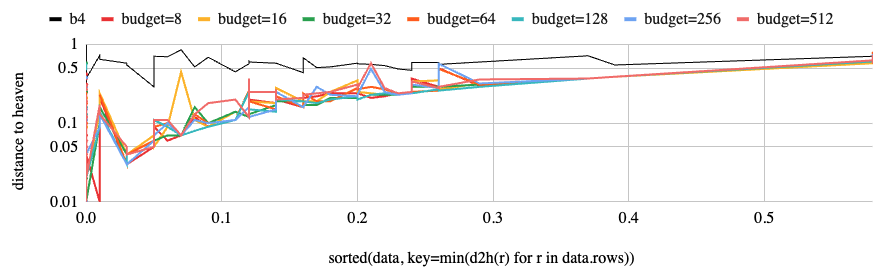
\includegraphics[width=.7\textwidth]{rands.png}\hspace{5mm}
\includegraphics[width=.25\textwidth]{bc.png}
\end{figure*}
 When faced with such a problem,  
 
% =========

  
% We seek simple methods for AI. Such tools, based on symbolic methods (decision trees, Bayes classifiers, K-means clustering, etc.), sometimes serve  as baselines that document the superiority of large language model (LLMs)-based approaches. But more  often,   we find they run 100x–1000x faster~\cite{majumder2018500+,ganguly2025lowgodatalightse} while matching the state-of-the-art.

% Not all AI tasks can be simplified; e.g. 
% generative tasks need require LLMs. But for the 120+ tasks examined here, symbolic methods produce code that is concise, explainable, verifiable, and teachable.


%  To say the least, there is little current work on simpler AI.
%  Much of  the software industry and 
% current software research is focused  on complex, resource intensive, AI models. As of 2026,  
% few-shot prompting \cite{chen2021evaluating, ouyang2022training} has evolved into
% holistic agentic workflows where LLMs
% with trillions of parameters,  used for 
%  multi-agent collaboration and
% repository-scale comprehension \cite{ma2023scope, wang2022machine,DBLP:journals/corr/abs-2507-15003,DBLP:journals/corr/abs-2509-06216,
% Dong2025SurveyCodeAgents}. Evolution
% from bidirectional models (BERT, CodeT5)
% \cite{devlin2018bert, feng2020codebert, wang2021codet5} to
% mixture-of-Experts and decoder-only models
% \cite{Lozhkov2024StarCoder2, DeepSeekAI2024DeepSeekCoderV2} enabled
% systems like DeepSeek-Coder-V2 and Llama 4 with massive context windows
% to navigate very large  codebases \cite{DBLP:conf/nips/YangJWLYNP24,
% DBLP:conf/issta/0002RFR24}, orchestrate tool workflows
% \cite{Rasheed2025AutonomousAgents} in order to  manage much of the   software development lifecycle.
% % %Paradigms include stateless pipelines
% % \cite{DBLP:journals/corr/abs-2407-01489}, flexible frameworks
% % \cite{DBLP:conf/iclr/0001LSXTZPSLSTL25}, and unified agents
% % \cite{DBLP:journals/corr/abs-2506-14683}.



% But while much has been {\em done}, it is not clear if it has been {\em done well}, or {\em done better} than alternate methods.  Table~\ref{cautions} catalogs known issues with LLMs. Some of these studies are a few years old, so some issues may have been resolved. But LLMs remain a fledgling technology, and given the costs of building new models or running large-scale verification studies, we simply cannot tell whether these are lingering problems or symptoms of a novel technology being rushed prematurely into widespread adoption.




% If complex LLM models are far from perfect, then can we use simpler methods?
%  This principle has deep roots.
%  Ptolemy (130 A.D.) urged explaining phenomena by "the simplest hypothesis possible," and William of Occam later cautioned that "entities must not be multiplied beyond necessity."  
% The benefits of simplicity are well-documented: reduced compute usage, lower energy costs~\cite{calrero15}, decreased pollution from energy production~\cite{monserrate2022cloud}, easier explanation~\cite{veerappa2011understanding}, faster tuning~\cite{fu2016tuning}.
%  Rudin~\cite{rudin2019stop}   argues  convincingly for the use of simpler system to obtain more trustworthy results:
% \begin{quote}
% {\em ``Stop explaining black box machine learning models for high stakes decisions and use interpretable models instead.''}
% \end{quote}
% Cognitive psychologists remark that interpretable models must not be large~\cite{gigerenzer2008heuristics,czerlinski1999good,phillips2017FFTrees}.
% Fortunately, as seen in Table~\ref{less}, 
%   the history of computing shows that  many complex systems  (including those doing inference) can be made much simpler.

% Despite all this work on simplicity, comparisons between LLM-based approaches and simpler alternatives remain rare in the SE literature. A recent survey of 229 SE papers using LLMs found only 5\% compared against a simpler baseline~\cite{Hou24} — a methodological gap, since simpler methods can be both faster and more accurate~\cite{grinsztajn2022why,somvanshi2024survey,Tawosi23,majumder2018500+,Ling24,Fu17,johnson2024ai}.




% We conjecture that this gap reflects a cognitive bias toward complexity. Adams and Fillon et al.~\cite{adams2021people,Fillon25} showed in 400+ human subjects given design tasks, people preferred additive over subtractive changes at a 4:1 ratio — {\em humans needlessly complicate their designs}.

 

% How to fix this? Perhaps what is missing are compelling exemplars showing the value of concise symbolic methods. This paper offers such exemplars via EZR, a compact Python toolkit addressing 120+ SE tasks: a core module of ~300 lines supporting a collection of application modules of ~60 lines each.
% A striking finding emerged during development: the underlying machinery is almost entirely shared across seemingly disparate tasks:
% \begin{itemize}
% \item Coding a nearest-neighbor classifier provided nearly everything needed for stochastic optimization (mutation, surrogate modeling, candidate evaluation).
% \item
% Similarly, coding an optimizer provided nearly everything needed for software configuration and performance tuning.
% \end{itemize}This convergence suggests a radical reframing: rather than a sprawling zoo of specialized algorithms, AI may reduce to a handful of core operations, with each "different" technique merely a thin variation on the same kernel. If so, the field has been making things harder than they need to be,  and EZR is an existence proof that a simpler foundation is both possible and practical.





% Why is there not more work on simplicity? Perhaps it is a cognitive bias. 

\noindent
Software engineers build tools that others can use. As far back as 1968, Doug McIlroy called for a shift in programming culture towards a ``tool-oriented'' approach based around   reusable  composable, and adaptable tools that can be mixed and matched as required.

\begin{quote} 
{\em We should expect the emergence of a family of standard parts, each individually repairable and 
replaceable, and plug-compatible with the rest~\cite{mcilroy1968mass}.} 
\end{quote}
 

Sadly, for the students we teach today in graduate classes.  that vision seems lost.
Based on a recent survey of our faculty colleagues, we find that far too many graduate students struggle to build tools that others can use. One student, for example, implemented a promising research prototype—but packaged it as an Eclipse-only plugin, locking out users who weren't already steeped in that ecosystem. A simple shell script {\one} would have made the tool vastly more accessible.
\circledblack
\begin{lstlisting}
def guess(data, budget=50, a=4):
  rows = shuffle(data.rows[:])
  seen = rows[:a]      # (*@\one@*) 
  todo = rows[a:]      # (*@\two@*)
  return seen, todo    # (*@\three@*)
\end{lstlisting} 
\circledtoggle
\begin{lstlisting}
def guess(data, budget=50, a=4): 
  rows = shuffle(data.rows[:])
  seen = rows[:a]      # (*@\one@*) 
  todo = rows[a:]      # (*@\two@*)
  return seen, todo    # (*@\three@*)
\end{lstlisting} 

This lack of tool-building fluency starts early. While judging  a recent high school hackathon, we saw that many teams submitted intentionally unusable “anti-productivity” tools, filled with popups and CAPTCHA traps. Their work was clever in concept, but defeatist in spirit—as if they had  already given up on building software that helps anyone else.

Part of the blame may lie with the current AI landscape.
Tools using large language models (LLMs)  like ChatGPT and Copilot have led students to assume that real SE tools can only be built by tech giants.

We think it’s time to correct that misconception.


We hence propose teaching {\IT}, a minimal scripting toolkit that empowers students to build their own efficient, composable AI tools for tasks like classification, regression, optimization, and text mining. Through assignments built around {\IT}, students rediscover the power of small, elegant tools—and see that (sometimes) simple methods can hold their own against massive models with massive budgets.

 




\subsection{Caveats}
Our goals are lofty, but realistic
While {\IT} is effective for many tasks, for purely generative
tasks, the best approach may sill  be an LLM~\cite{gros2020code}. 

That said, what we seek to engender in students is an    mindset   that uses other people's complex tools which necessary, and simpler tools for everything else.
And there often much simpler and faster approaches than LLMs.   
E.g. in a recent   review~\cite{Hou24} of 229 SE papers using large language models,  only $13/229 \approx 5\%$ of those papers compared LLMs to other approaches. This is a methodological error
since   other methods  can
 produce results that are better and/or 
faster~\cite{grinsztajn2022why,somvanshi2024survey,Tawosi23,majumder2018500+,Ling24,Fu17,johnson2024ai}.   

\section{Motivation}
Just to motivate  this work, this section gives some examples of EZR in action.
The two main thing to take from these examples is that:
\begin{itemize}
\item
For many software engineering
applications, surprisingly small models can be surprisingly effective.
\item
  Under the hood, symbolic AI tools share many core algorithms 
and data structures. That is, if engineered correctly, after building one such tool,
many more are just small extension. 
\end{itemize}

Table~\ref{jpl} shows a sample of 10,000 rows generated  from a simulator exploring software
product/ process/ personnel options for the Orbital Space Plan  software project
fro the Jet Propulsion Laboratory.
 EZR's {\tt xplain} tool summarizes csv files like Table~\ref{jpl} as follows:
\begin{itemize}
\item Find  each row's  $Y_i$: the   Euclidean distance to least estimated effort, defects, risks, and months. {\em Smaller}   $Y_i$ values
are {\em better}.
\item Discretizes each row's $x$ values; e.g. KLOC (lines of code)
could be divided into $B=5$ bins: very low, low, mid, high, very high.
\item  Scores  bins by $\Sigma Y_i$ for all  $\mathit{row_i} \in \mathit{rows}$ having that bin.
\item Sorts   $x$ attribute by bin score  variability (since
high variance means attributes  can select for best/worst project options).
\end{itemize}
Figure~\ref{jpl} shows  {\tt xplain}'s output.  In that figure
\color{red}{\bf RED}\color{black}~ 
and  \color[RGB]{0,140,0}{\bf GREEN}\color{black}~ shows worst and best bins.
Note that most attributes have flat bin scores; i.e. for the purposes
of minimizing the $y$ dependent goals of Table~\ref{jpl}, they are not useful.
\begin{figure}
\begin{center}
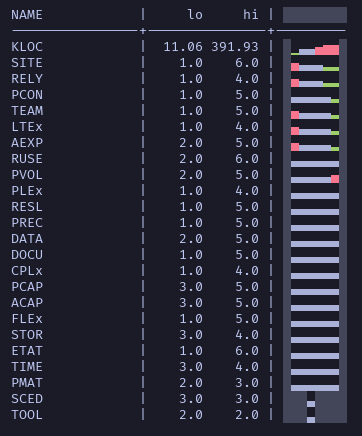
\includegraphics[width=2in]{xplain_osp.png}
\end{center}
\caption{EZR's {\em xplain} tool
finds influence  ranges inside  the JPL orbital space plane project.
A sample of that  data  of that was shown in  Table~\ref{jpl}
Here, attributes are   divided into $B=7$ bins. 
}\label{xplain}
\end{figure}

EZR's {\em xplainr} tool takes this figure and build rules by exploring
subsets of the   better
 ranges. Given $M$ best bins, {\em explainr}:xxxx


not useful.
\begin{figure}
\begin{center}

\includegraphics[width=2in]{bc.png}
\end{center}
\caption{EZR's {\em tree} tool. 200 calls, 127 data sets,  ransom select of training instances,  selecting
$25 \le B \le 200$
and 
$3\le C \le 6$ at random,
then running 20 repeats. Each pixel's value is a weighted average of all data points, where weight is
$ 1/d^2$.
}\label{xplain}
\end{figure}


\subsection{Is Simpler Possible?}

Artificial intelligence (AI) is often perceived as complex, compute-intensive, energy-hungry, and opaque. These characteristics—common in modern deep learning systems—can be particularly discouraging in educational settings, where transparency, responsiveness, and simplicity are paramount. As a result, AI is frequently perceived as too complex to understand-- wwhich has negagive consqueneces

as a theoretical subject, divorced from practical experimentation with real tools.

Yet this black-box, big-data view of AI overlooks a long tradition in machine learning and statistics that shows most data is not useful for a given task. Techniques such as principal component analysis, information gain pruning, and recent work on data backdoors all point to the same conclusion: much of the data can safely be discarded without harming (and often improving) performance. This raises a provocative question: what if we built AI tools assuming that most data is irrelevant?

This paper presents a lightweight AI toolbox designed around that assumption. By embracing active learning, incremental updates, and stochastic sampling, we show that a substantial portion of traditional AI complexity can be eliminated. Under the hood, this system includes several engineering choices—such as streaming Bayesian learners and recursive diversity sampling—that yield dramatic speedups (e.g., 100–1000× compared to baseline full-data approaches) while maintaining clarity and pedagogical value.

The result is a compact, fast, and understandable AI toolkit suitable for teaching and experimentation, without sacrificing performance. This paper reports on the design choices, core algorithms, and classroom experiences using this system in graduate-level courses.



Please lay out your article using the section headings and the given body text is dummy text for layout purpose.
Lorem ipsum dolor sit amet, consectetuer adipiscing elit \cite{Hirt1974}. Ut purus elit, vestibulum ut, placerat ac, adipiscing vitae,
felis. Curabitur dictum gravida mauris. Nam arcu libero, nonummy eget, consectetuer id, vulputate a, magna. Donec
vehicula augue eu neque. Pellentesque habitant morbi tristique senectus et netus et malesuada fames ac turpis egestas.
Mauris ut leo. Cras viverra metus rhoncus sem. Nulla et lectus vestibulum urna fringilla ultrices. Phasellus eu tellus
sit amet tortor gravida placerat. Integer sapien est, iaculis in, pretium quis, viverra ac, nunc. Praesent eget sem vel
leo ultrices bibendum. Aenean faucibus. Morbi dolor nulla, malesuada eu, pulvinar at, mollis ac, nulla. Curabitur
auctor semper nulla. Donec varius orci eget risus. Duis nibh mi, congue eu, accumsan eleifend, sagittis quis, diam.
Duis eget orci sit amet orci dignissim rutrum.


\section{Design Principles}\label{sec2}

Eric's rule: data before functions.

Uncle Bob's rule: Robert Martin 5 lives on code

No to OO. This code uses polymorphsim (different data types resont to command in their own way) but not objects. The itnally code base was writen in Luas where it is possible to define methods in any order. But puthonr esists that. so we coud be can but tother things that go toehter if we use fuction. Yes , this means that 3-4 times it uses a switchs tatement to process different types. Implememted using PPything's temamary peprators, these swotches are not parcaulr clusmy (just  1 to 3 lines to code. also the less hatton experience.

%\nocite{*}% Show all bib entries - both cited and uncited; comment this line to view only cited bib entries;

\bibliography{main,bib2} 
\bibliographystyle{wileyNJD-AMA} 

\bmsection*{Author Biography}

\begin{biography}{
\includegraphics[width=76pt,height=76pt,draft]{empty}}{
{\textbf{Author Name.} Please check with the journal's author guidelines whether
author biographies are required. They are usually only included for
review-type articles, and typically require photos and brief
biographies for each author.}}
\end{biography}


\end{document}
